%%%%%%%%%%%%%%%%%%%%%%%%%%%%%%%%%%%%%%%%%%%%%%%%%%%%%%%%%%%%%%%%%%%%%%%%%%%%%%
% Trabalho Java RMI de Desenvolvimento de Aplicações Móveis e Distribuídas
%%%%%%%%%%%%%%%%%%%%%%%%%%%%%%%%%%%%%%%%%%%%%%%%%%%%%%%%%%%%%%%%%%%%%%%%%%%%%%
\documentclass[12pt,brazil, a4paper, fullpage]{article}

%%%%%%%%%%%%%%%%%%%%%%%%%%%%%%%%%%%%%%%%%%%%%%%%%%%%%%%%%%%%%%%%%%%%%%%%%%%%%%
% Preambulo - Configuração de página
%%%%%%%%%%%%%%%%%%%%%%%%%%%%%%%%%%%%%%%%%%%%%%%%%%%%%%%%%%%%%%%%%%%%%%%%%%%%%%
%%%%%%%%%%%%%%%%%%%%%%%%%%%%%%%%%%%%%%%%%%%%%%%%%%%%%%%%%%%%%%%%%%%%%%%%%%%%%%
% Preambulo - Pacotes
%%%%%%%%%%%%%%%%%%%%%%%%%%%%%%%%%%%%%%%%%%%%%%%%%%%%%%%%%%%%%%%%%%%%%%%%%%%%%%
\usepackage[table]{xcolor}
\usepackage{geometry}
\usepackage[portuges]{babel}
\usepackage[portuges]{translator}
\usepackage[T1]{fontenc}
\usepackage[utf8]{inputenc}
\usepackage{epsfig}
\usepackage{multirow}
\usepackage{tikz}
\usepackage{listings}
\usepackage{natbib}
\usepackage{hyperref}
\usepackage{multicol}
\usepackage{fancyhdr}
\usepackage{enumitem}

%%%%%%%%%%%%%%%%%%%%%%%%%%%%%%%%%%%%%%%%%%%%%%%%%%%%%%%%%%%%%%%%%%%%%%%%%%%%%%
% Preambulo - Configuração de Página
%%%%%%%%%%%%%%%%%%%%%%%%%%%%%%%%%%%%%%%%%%%%%%%%%%%%%%%%%%%%%%%%%%%%%%%%%%%%%%
\setlength{\topmargin}{0pt}
\setlength{\voffset}{-1.8cm}
\setlength{\textheight}{25,6cm}
\setlength{\oddsidemargin}{0cm}
\setlength{\evensidemargin}{0cm}
\setlength{\hoffset}{-1cm}
\setlength{\textwidth}{18cm}

\pagestyle{empty}

\input xy
\xyoption{all}
\xyoption{color}



%%%%%%%%%%%%%%%%%%%%%%%%%%%%%%%%%%%%%%%%%%%%%%%%%%%%%%%%%%%%%%%%%%%%%%%%%%%%%%
% Define cabeçalho de prova
%%%%%%%%%%%%%%%%%%%%%%%%%%%%%%%%%%%%%%%%%%%%%%%%%%%%%%%%%%%%%%%%%%%%%%%%%%%%%%
\newcommand{\cabecalhoProva}{
\pagestyle{fancy} % define página com cabeçalho
\fancyhf{} % limpa todos os cabeçalhos e rodapés
\setlength{\headheight}{22pt} %% define tamanho personalizado de cabeçalho
\renewcommand{\headrulewidth}{0pt} % elimina a linha de separação do cabeçalho
\fancyhead[LO]{\dadosAluno}
}


%%%%%%%%%%%%%%%%%%%%%%%%%%%%%%%%%%%%%%%%%%%%%%%%%%%%%%%%%%%%%%%%%%%%%%%%%%%%%%
% Logo da PUC Minas
%%%%%%%%%%%%%%%%%%%%%%%%%%%%%%%%%%%%%%%%%%%%%%%%%%%%%%%%%%%%%%%%%%%%%%%%%%%%%%
\newcommand{\logoPUC}[2]{
\begin{center}\renewcommand{\tabcolsep}{3mm}
    \begin{tabular*}{\textwidth}{ll}
        \multirow{4}{*}{\includegraphics[height=1.4cm]{#2}}
        &   \\
        & \usefont{T1}{cmss}{bx}{n} PONTIFÍCIA  UNIVERSIDADE  CATÓLICA  DE  MINAS  GERAIS  \\
        &  \usefont{T1}{cmss}{bx}{n} #1\vspace{2mm}\\
        &   \\
    \end{tabular*}
\end{center}
}

%%%%%%%%%%%%%%%%%%%%%%%%%%%%%%%%%%%%%%%%%%%%%%%%%%%%%%%%%%%%%%%%%%%%%%%%%%%%%%
% Caracteristicas da disciplina
%%%%%%%%%%%%%%%%%%%%%%%%%%%%%%%%%%%%%%%%%%%%%%%%%%%%%%%%%%%%%%%%%%%%%%%%%%%%%%

\newcommand{\dadosDisciplina}[5]{
\begin{center}
\begin{tabular*}{\textwidth}{|p{7.5cm}@{\extracolsep{\fill}}|p{5.5cm}|p{2cm}|p{1.2cm}|}
    \hline
    \sf Disciplina & \sf Departamento & \sf Turno & \sf Período \\
    
    \multicolumn{1}{|c|}{#1} &
    \multicolumn{1}{c|}{#2} &
    \multicolumn{1}{c|}{#3} &
    \multicolumn{1}{r|}{#4$^\circ$} \\ \hline \hline
    \multicolumn{4}{|l|}{\sf Professor} \\
    \multicolumn{4}{|l|}{\hspace{1cm} #5} \\ \hline
\end{tabular*}
\end{center}
}


\newcommand{\dadosAluno}{
\begin{tabular*}{\textwidth}{|p{.2\textwidth}@{\extracolsep{\fill}}|p{.75\textwidth}|}
	\hline
	\sf Matrícula: & \sf Aluno: \\
	\hspace{1cm} & \hspace{1cm} \\
	\hline
\end{tabular*}
}


%%%%%%%%%%%%%%%%%%%%%%%%%%%%%%%%%%%%%%%%%%%%%%%%%%%%%%%%%%%%%%%%%%%%%%%%%%%%%%
% Título simples
%%%%%%%%%%%%%%%%%%%%%%%%%%%%%%%%%%%%%%%%%%%%%%%%%%%%%%%%%%%%%%%%%%%%%%%%%%%%%%
\newcommand{\tituloPUC}[1]{
\vspace{3mm}

\begin{center}
    {\Large \bf #1}
\end{center}

\vspace{3mm}
}



%%%%%%%%%%%%%%%%%%%%%%%%%%%%%%%%%%%%%%%%%%%%%%%%%%%%%%%%%%%%%%%%%%%%%%%%%%%%%%
% Comandos para gabarito
%%%%%%%%%%%%%%%%%%%%%%%%%%%%%%%%%%%%%%%%%%%%%%%%%%%%%%%%%%%%%%%%%%%%%%%%%%%%%%
\newcommand{\itemvf}[1]{\item ( \ifgabarito  #1 \else\hspace{8mm}\fi )}
\newcommand{\itemresp}[1]{\ifgabarito \textbf{\item #1} \else \item #1 \fi}


\usepackage{booktabs}
\usepackage{wrapfig}


%%%%%%%%%%%%%%%%%%%%%%%%%%%%%%%%%%%%%%%%%%%%%%%%%%%%%%%%%%%%%%%%%%%%%%%%%%%%%%
% Inicio do documento
%%%%%%%%%%%%%%%%%%%%%%%%%%%%%%%%%%%%%%%%%%%%%%%%%%%%%%%%%%%%%%%%%%%%%%%%%%%%%%
\begin{document}

    \selectlanguage{brazil}
    \lstset{language=Java,
        basicstyle=\small, % print whole listing small
        showstringspaces=false}

%%%%%%%%%%%%%%%%%%%%%%%%%%%%%%%%%%%%%%%%%%%%%%%%%%%%%%%%%%%%%%%%%%%%%%%%%%%%%%
% Logo da PUC Minas
%%%%%%%%%%%%%%%%%%%%%%%%%%%%%%%%%%%%%%%%%%%%%%%%%%%%%%%%%%%%%%%%%%%%%%%%%%%%%%
\thispagestyle{plain}
\logoPUC{Curso de Bacharelado em Engenharia de Software}{puc_engesoft_logo.png}

%%%%%%%%%%%%%%%%%%%%%%%%%%%%%%%%%%%%%%%%%%%%%%%%%%%%%%%%%%%%%%%%%%%%%%%%%%%%%%
% Caracteristicas da disciplina
%%%%%%%%%%%%%%%%%%%%%%%%%%%%%%%%%%%%%%%%%%%%%%%%%%%%%%%%%%%%%%%%%%%%%%%%%%%%%%
\dadosDisciplina{Lab. Desenv. Aplic. Móveis e Distribuídas}{Engenharia de Software}{Noite}{5}{Hugo de Paula (hugo@pucminas.br)}

\tituloPUC{Trabalho de Spring MVC –- Home Broker}


%%%%%%%%%%%%%%%%%%%%%%%%%%%%%%%%%%%%%%%%%%%%%%%%%%%%%%%%%%%%%%%%%%%%%%%%%%%%%%
% Corpo
%%%%%%%%%%%%%%%%%%%%%%%%%%%%%%%%%%%%%%%%%%%%%%%%%%%%%%%%%%%%%%%%%%%%%%%%%%%%%%

\section{Objetivos do trabalho}

O objetivo deste trabalho é desenvolver uma aplicação simples baseada no framework back-end Java Spring.

\section{Especificação}

\indent \indent Considere a arquitetura Spring a seguir:

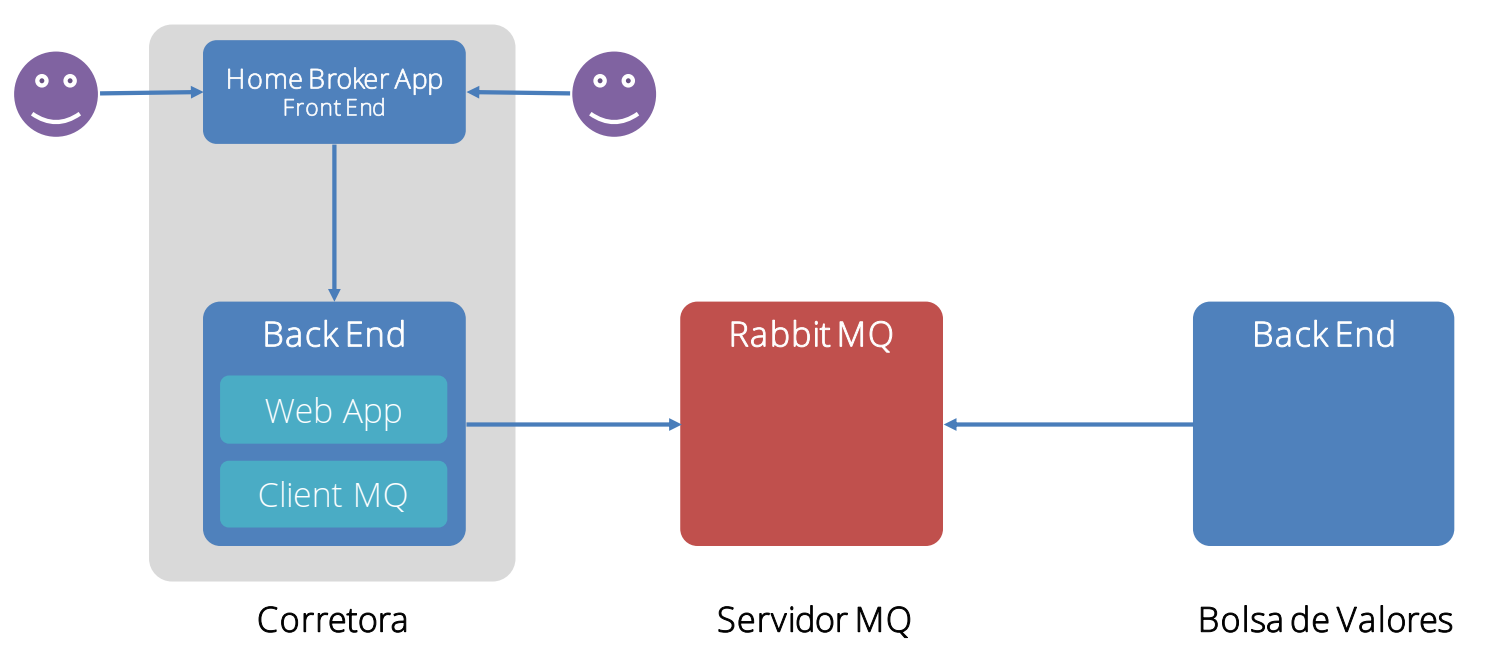
\includegraphics[width=\textwidth]{mvc-architecture.png}


O trabalho consiste na construção de uma aplicação completa que oferece uma interface de home broker e operacionaliza a negociação de ativos em uma bolsa de valores.

A aplicação consiste em três módulos principais:

\begin{enumerate}
    \item Corretora:
\begin{enumerate}
    \item Uma aplicação web que proporciona uma interface para os usuários realizarem login.
    \item Após o login, os usuários podem visualizar os ativos disponíveis para negociação.
    \item Este módulo é responsável por permitir que os usuários enviem ordens de compra e venda para o servidor de mensageria (Servidor MQ).
\end{enumerate}
    \item Servidor MQ:
\begin{enumerate}
    \item Recebe todas as requisições provenientes do módulo Corretora.
    \item Interage com o módulo da Bolsa de Valores para comunicar os pedidos de transações.
    \item Responsável por processar e rotear as ordens recebidas para a Bolsa de Valores e retornar as transações realizadas para que sejam repassadas à
Corretora.

\end{enumerate}
    \item Bolsa de Valores:
\begin{enumerate}
    \item Possui um livro de ofertas e armazena todas as transações realizadas.
    \item Interage com o módulo do Servidor MQ para receber pedidos de compra e venda.
    \item Processa os pedidos recebidos, executa as transações correspondentes e retorna os resultados ao Servidor MQ para serem repassados à Corretora.

    \end{enumerate}
\end{enumerate}

Este sistema proporciona aos usuários a capacidade de visualizar e negociar ativos na bolsa de valores de forma eficiente, com a corretora atuando como intermediária entre os usuários e a bolsa de valores. O Servidor MQ desempenha um papel crucial na comunicação entre a Corretora e a Bolsa de Valores, garantindo uma troca eficaz de informações e a execução precisa das transações.

\section{Resultados Esperados}

Deverá ser entregue:

\begin{enumerate}
    \item Todo o código, comentado.

    \item Um arquivo README.TXT contendo uma explicação sucinta do código e instruções para compilação e execução do mesmo.
\end{enumerate}


\end{document}
